\documentclass[9pt]{exam} 
\addpoints
\pointsinmargin

\usepackage[fleqn]{amsmath}
\usepackage{amssymb} %standard classy maths symbols
\usepackage[a4paper, margin=1in]{geometry} %makes it easy to specify where to put stuff on the page

\usepackage{tcolorbox} % basic but good package for boxes around text
\tcbset{colback=black!5!white}

\usepackage{tikz} % interval diagrams, sets, etc.

\begin{document}

\textbf{Name:} \dotfill



\begin{questions} 
\question Let $P$, $Q$, $R$ and $S$ be points in the plane.

\begin{parts}
\part[2] Which of the following objects represent a vector? \hfill \emph{Tick the boxes.}

$\hfill \square \,\, P \hfill \square \,\, [PQ] \hfill \square \,\, \overrightarrow{PQ} \hfill \square \,\, \overrightarrow{QP} \hfill \square \,\, PQR \hfill $



\fullwidth{
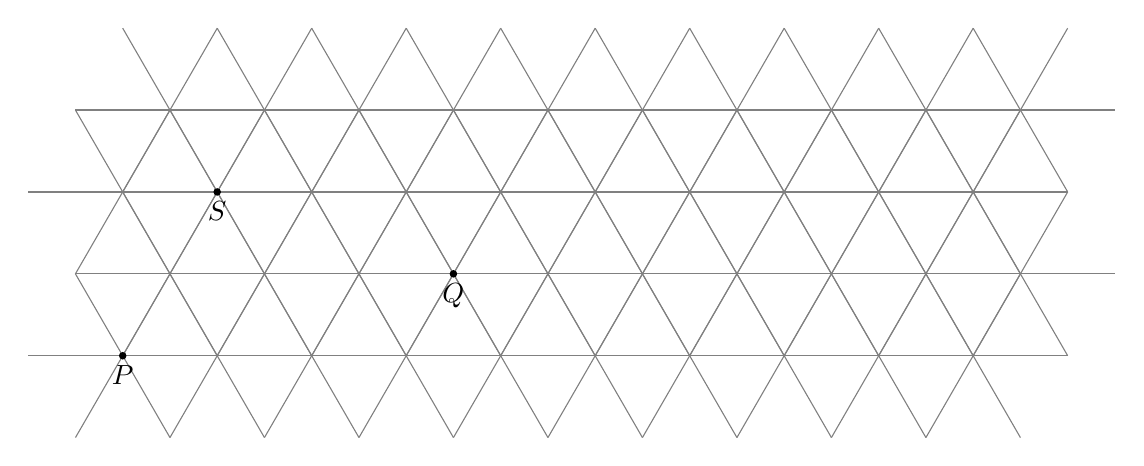
\begin{tikzpicture}[scale=0.8]
  \foreach \x in {0,...,9} {
    \foreach \y in {0,1} {
      \coordinate (a) at (\x*1.5, \y*2.6);
      \coordinate (b) at (\x*1.5 + 0.75, \y*2.6 + 1.3);
      \foreach \z in {0,1,2,3,4,5} {
        \draw[gray] (a) -- ++(\z*60:1.5);
        \draw[gray] (b) -- ++(\z*60:1.5);
      }
    }
  }
  
  \fill (0, 0) circle (0.6mm) node[below] {$P$};
  \fill (5.25, 1.3) circle (0.6mm) node[below] {$Q$};
  \fill (1.5, 2.6) circle (0.6mm) node[below] {$S$};
\end{tikzpicture}
}

\part[1] Draw the arrows  $\overrightarrow{PS}$ and $\overrightarrow{PQ}$ on the plane above.

\part[1] Given that $\overrightarrow{PS} = \overrightarrow{QR}$, mark the point $R$ on the plane above.

\part[1] What is the nature of the quadrangle $PQRS$? \dotfill

\part[1] $\overrightarrow{PS} + \overrightarrow{PQ} = \ldots$

$\hfill \square \,\, \overrightarrow{PS}  \hfill \square \,\, \overrightarrow{0}  \hfill \square \,\, \overrightarrow{SR} \hfill \square \,\, \overrightarrow{QP} \hfill \square \,\, \overrightarrow{PR}  \hfill $

\

\part[1] Mark the new point $V$ on the plane, given that $\overrightarrow{PV} = 2 \cdot \overrightarrow{PQ}$. 

\part[1] Which other arrow has the same size and direction as $\overrightarrow{VQ}$? \dotfill

\end{parts}

\question[5] The vector $\overrightarrow{s}$ is directed due north and $\| \overrightarrow{s} \|  = 6$.  
The vector $\overrightarrow{t}$ is directed due west and $\| \overrightarrow{t} \|  = 8$. 
Find $\| \overrightarrow{s}  + \overrightarrow{t}\|$.
\fillwithdottedlines{5cm}

\vfill

\question[0] \textbf{Bonus.} Let $\overrightarrow{WX} = \overrightarrow{a}$, $\overrightarrow{WY} = \overrightarrow{b}$, and $\overrightarrow{WZ} = \overrightarrow{c}$. It is given that $\overrightarrow{XY} = \overrightarrow{YZ}$.

Prove that $\overrightarrow{a} + \overrightarrow{c} = 2 \cdot \overrightarrow{b}$. \hfill \emph{Work on the back.}

\end{questions}


\begin{tcolorbox}

\textbf{Name of marker:}

\begin{center}
\gradetable[h][questions]
\end{center}

\end{tcolorbox}


\end{document}